\documentclass[dvipsnames,tikz]{standalone}
\usepackage{amsmath}
\usepackage{arevmath}
\usepackage{xcolor}
\usepackage{tikz}
\usetikzlibrary{calc}
\usetikzlibrary{decorations.pathreplacing,calligraphy,3d}
\usepackage{tikz-3dplot} 

\tikzset{main/.style={thick, circle, color=black}}

\newcommand{\arrowIn}{
	\tikz \draw[-stealth] (-1pt,0) -- (1pt,0);
}

\begin{document}
	
	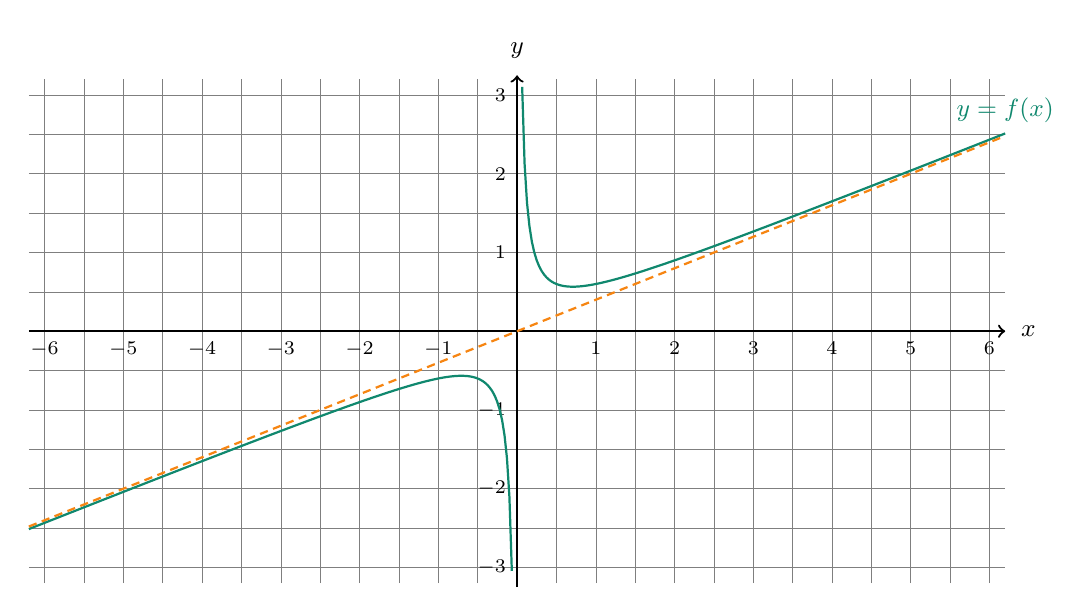
\begin{tikzpicture}[font=\small, tl/.style = {black, inner sep=1pt, font=\scriptsize} ]
		% grid
		\draw[main, very thin, xstep=0.5, ystep=0.5, semitransparent] (-6.2,-3.2) grid (6.2,3.2);
		
		% y tick label
		\foreach \y in {-3,-2,-1,1,2,3}{
			\node[tl,left=1mm] at (0,\y) {$\y$};
		}
		% x tick label
		\foreach \x in {-6,-5,-4,-3,-2,-1,1,2,3,4,5,6}{
			\node[tl,below=1mm] at (\x,0) {$\x$};
		}
		
		% curve
		\draw[thick,PineGreen,domain=0.065:6.2,variable=\x, samples=200] plot(\x,{(2*(\x)^2+1)/(5*\x)}) node [above] {$y=f(x)$};
		\draw[thick,PineGreen,domain=-6.2:-0.065,variable=\x, samples=200] plot(\x,{(2*(\x)^2+1)/(5*\x)});
		
		% axes
		\draw[main, ->,thick] (-6.2,0) -- (6.2,0) node[right] {$x$};
		\draw[main, ->,thick] (0,-3.25) -- (0, 3.25) node[above] {$y$};	
		
		\draw[thick, densely dashed,BurntOrange,domain=-6.2:6.2,variable=\x] plot(\x,0.4*\x);
	\end{tikzpicture}
\end{document}